\documentclass[tikz,border=12pt]{standalone}
\usepackage{amsmath,amssymb}
\usetikzlibrary{arrows.meta,calc}

\begin{document}
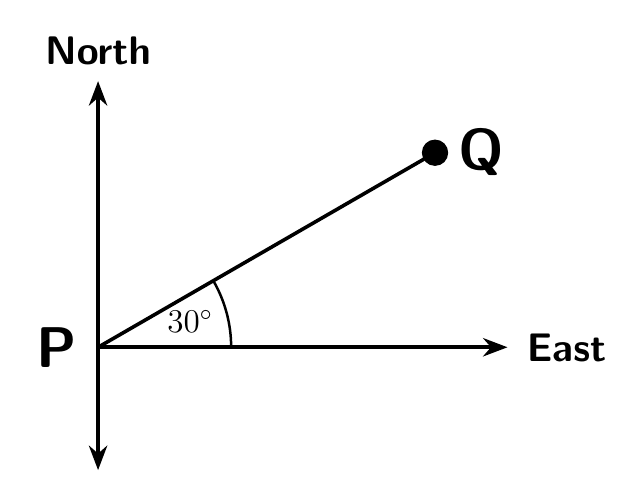
\begin{tikzpicture}[>=Stealth, scale=1.3]
    \coordinate (P) at (0, 0);
    
    % North-South vertical axis
    \draw[line width=1.3pt, <->] (0, -1.2) -- (0, 2.6) node[above=2pt, font=\Large\sffamily\bfseries] {North};
    
    % East horizontal axis
    \draw[line width=1.3pt, ->] (0, 0) -- (4.0, 0) node[right=3pt, font=\Large\sffamily\bfseries] {East};
    
    % Point P label
    \node[left=4pt, font=\huge\sffamily\bfseries] at (P) {P};
    
    % Ray to Q at 30 degrees elevation from East
    \def\ang{30}
    \def\len{3.8}
    \coordinate (Q) at ({\len*cos(\ang)}, {\len*sin(\ang)});
    
    \draw[line width=1.3pt] (P) -- (Q);
    \filldraw[black] (Q) circle (3.5pt) node[right=5pt, font=\huge\sffamily\bfseries] {Q};
    
    % Angle arc for 30 degrees (from 0 to 30)
    \draw[line width=0.9pt] ($(P) + (0:1.3)$) arc (0:\ang:1.3);
    \node[font=\large\bfseries] at (0.9, 0.25) {$30^\circ$};
    
\end{tikzpicture}
\end{document}
